\chapter{HASIL YANG DIHARAPKAN}

\section{Hasil yang Diharapkan dari Penelitian}

Dari penelitian yang akan dilakukan, diharapkan alat yang dihasilkan dapat mempermudah proses pengisian token listrik pada 
meteran prabayar secara otomatis dan nirkabel. Alat ini dirancang agar mampu menekan tombol-tombol pada meteran listrik dengan presisi tinggi, 
sesuai dengan angka yang dimasukkan melalui aplikasi kontrol melalui aplikasi web atau \textit{mobile}. Selain itu, alat ini diharapkan dapat dipasang secara fleksibel pada 
berbagai model meteran listrik prabayar, tanpa memerlukan modifikasi besar pada perangkat meteran listrik prabayar yang sudah ada.

Dengan dilengkapi sistem kamera dan mikrofon, alat ini juga memungkinkan pengguna untuk memverifikasi keberhasilan proses 
pengisian token secara visual dan auditori, serta memastikan token yang dimasukkan telah diterima dengan benar. Alat ini diharapkan 
tidak hanya meningkatkan efisiensi waktu dalam pengisian token tetapi juga memberikan kenyamanan dan keandalan bagi pengguna dalam 
memastikan proses berjalan tanpa gangguan. Dalam jangka panjang, alat ini dapat menjadi solusi yang hemat energi dan dapat diandalkan 
dalam pengelolaan listrik prabayar berbasis IoT.

\section{Hasil Pendahuluan}

Sampai saat ini, pembuatan alat pengisi token listrik dalam tahapan perancangan desain dan implementasi hardware, memastikan bahwa desain dan struktur dari alat
dapat memenuhi kebutuhan secara berat dan tetap mempertahankan presisi dari alat, desain juga sangat penting untuk memastikan alat terlihat baik secara estetika dan ergonomis.

Secara perangkat keras, penggerak vertikal dengan komponen stepper motor, lead screw, dan coupling sudah terpasang dan sudah bisa bergerak secara vertikal,
sistem ini dibantu dengan adanya guide rail yang dapat meningkatkan presisi dan mempermudah pergerakan dari load alat, dimana bagian ini akan mengerakkan
bagian alat yang bergerak secara horizontal serta bagian yang akan menekan tombol pada meteran listrik prabayar.
Selain itu, alat sudah bisa mengontrol motor vertikal dengan menggunakan program dengan menggunakan stepper motor driver TB6600 selama proses pengembangan dan akan diganti dengan stepper motor driver 
yang lebih kecil dan lebih hemat energi. Gambar \ref{fig:hasil-pendahuluan} adalah hasil sementara dari alat yang dibuat.

\newpage
\begin{figure}[H]
  \centering
  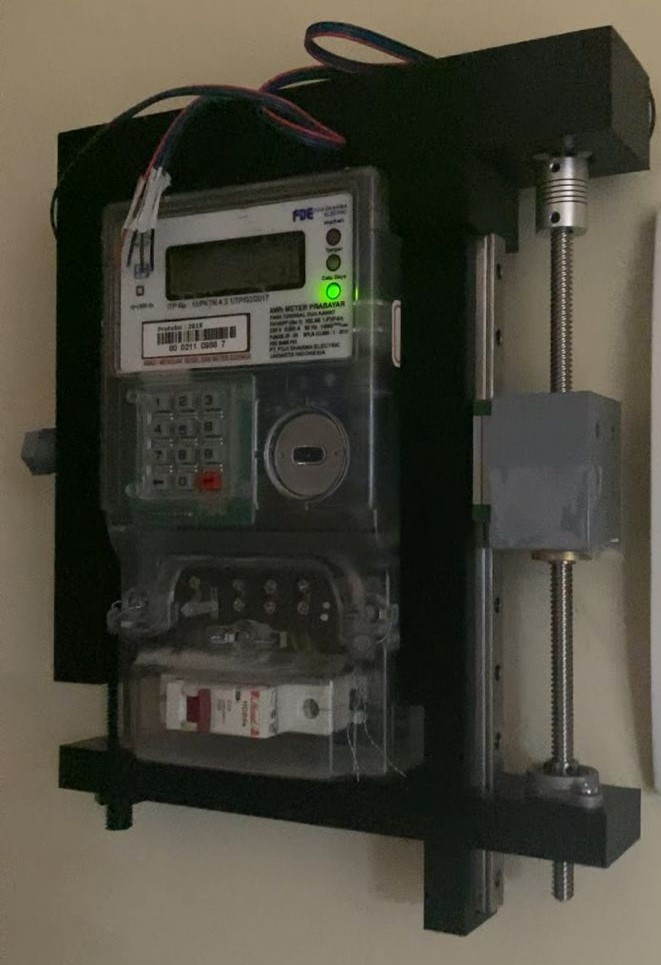
\includegraphics[width=0.4\textwidth]{gambar/hasil-pendahuluan.jpg}
  \caption{Hasil Pendahuluan}
  \label{fig:hasil-pendahuluan}
\end{figure}